% !TEX root = ../main.tex
\documentclass[../main.tex]{subfiles}

\begin{document}
\section{Computers and computer groups}

\subsection{Computers page}

Computer page show a list of computers in the system that are grouped into collapsable groups.
The page implementation can be found under \texttt{dashboard/ipxe/computers} in the
app router direcotry of the web interface application.

Most of the code is used for displaying the computer list with the support fo drag and drop computers between groups.
Drag and drop is implemented using the \texttt{dnd} library for React \cite{dnd}.

\begin{figure}[H]
  \centering
  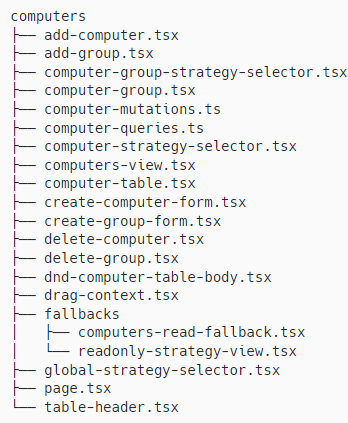
\includegraphics[width=0.5\textwidth]{file-tree/computers-table-file-tree.png}
  \caption{File tree of the computer page}
\end{figure}

\begin{figure}[H]
  \centering
  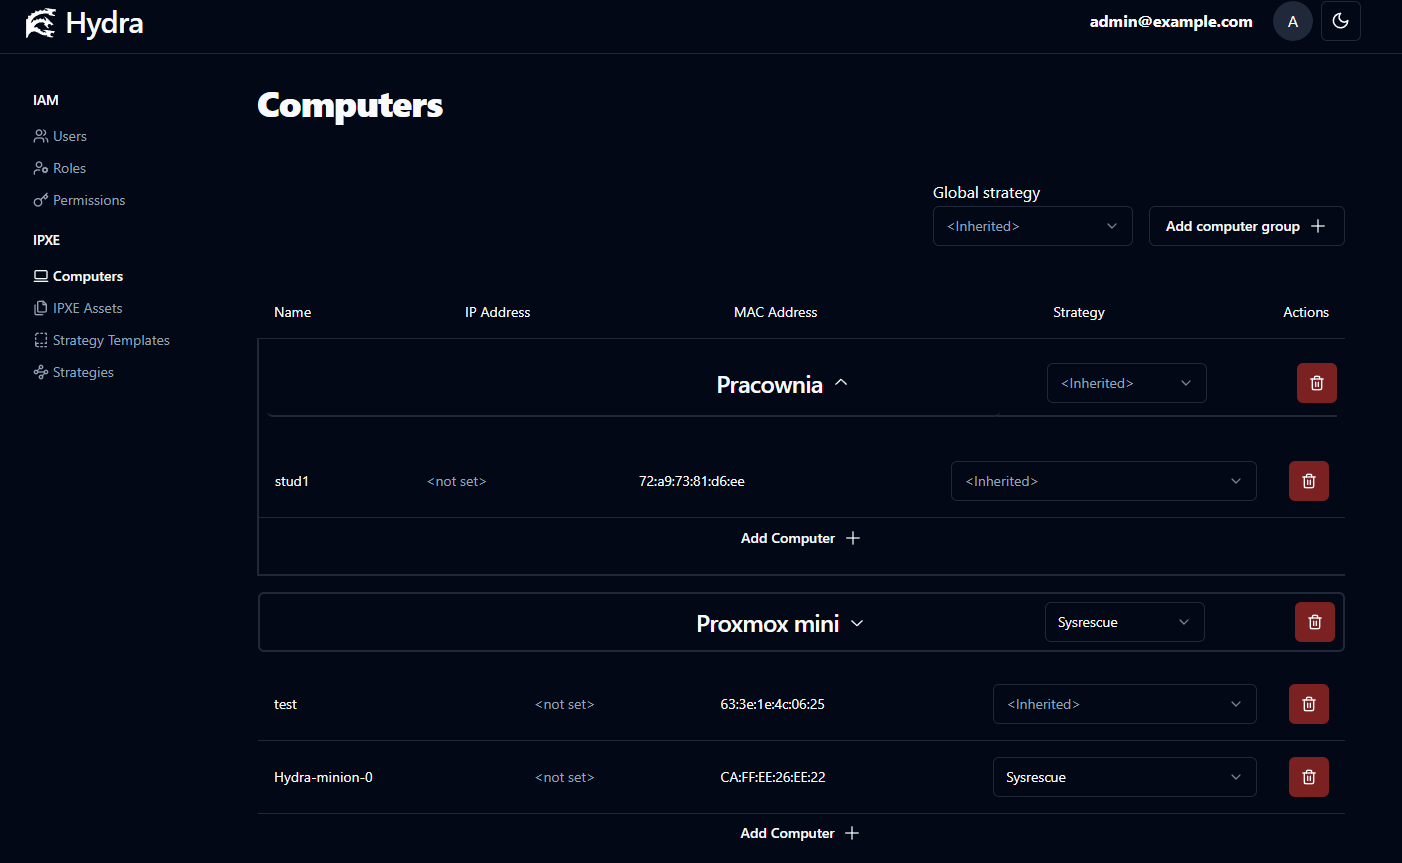
\includegraphics[width=\textwidth]{computers/computers-page.png}
  \caption{Computers page}
\end{figure}

In the fiure above, the first computer group is expanded, and the second one is collapsed. Computers without assigned group are displayed at the bottom of the list.
Computer entries are not able to be edited after they are added, they can be however deleted and added again.

To add a new computer, the user has to click on the \texttt{Add computer} button, which opens a model with a form to fill in the computer details.
Each computer group contains \texttt{Add computer} button, which adds a computer to the group. Clicking on the button ourside of the group adds a computer without a group.

\begin{figure}[H]
  \centering
  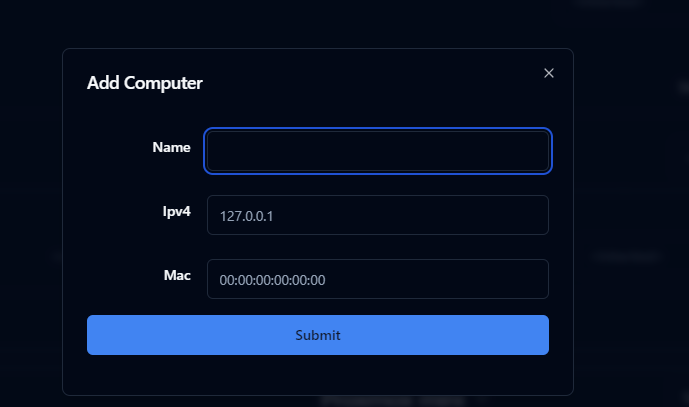
\includegraphics[width=0.6\textwidth]{computers/add-computer-modal.png}
  \caption{Modal with a form to add a new computer}
\end{figure}

Adding a computer group is simmilary done by clicking on the \texttt{Add computer group} button visible in the top part of the page.

\begin{figure}[H]
  \centering
  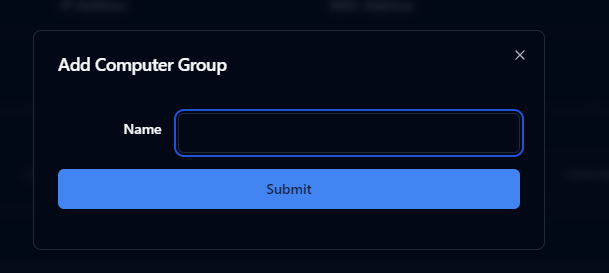
\includegraphics[width=0.6\textwidth]{computers/add-computer-group-modal.png}
  \caption{Modal for adding new computer group}
\end{figure}

To assign a computer to a group click and hold the computer entry and drag it to the desired group. The computer will be automatically assigned to the group.
A red border is shown around the group when the computer is dragged over it. The entries in the group will move to make space for the dragged computer.

\begin{figure}[H]
  \centering
  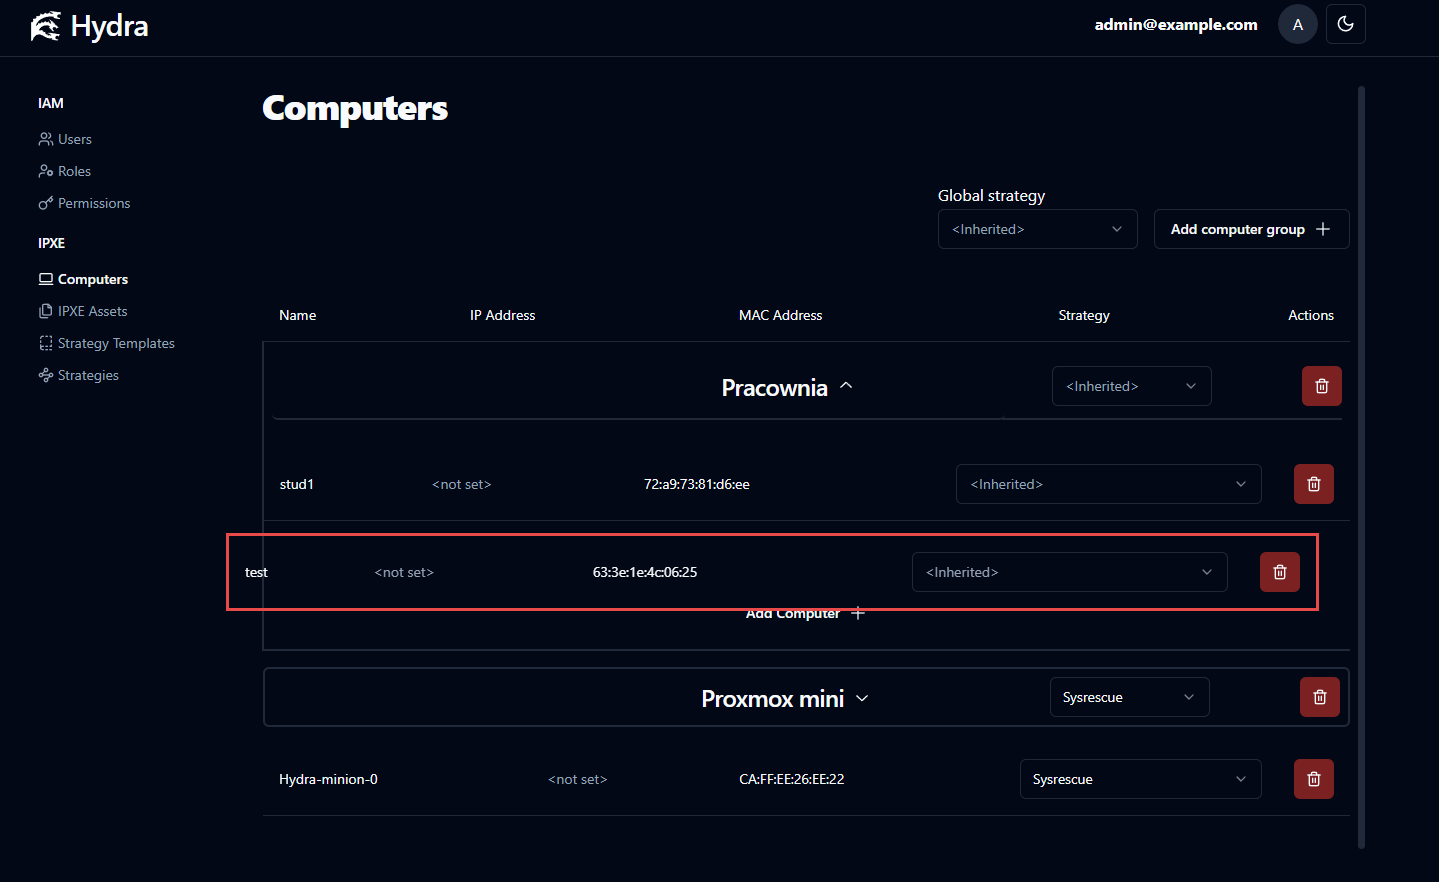
\includegraphics[width=\textwidth]{computers/drag-and-drop.png}
  \caption{Drag and drop in action}
\end{figure}

\subsection{GraphQL's queries and mutations for computer management}

The \texttt{ipxe} backend module offers the following queries and mutations for computer management.

\begin{listing}[H]
  \textfile{implementation/code/computers/queries.gql}
  \caption{GraphQL queries for computer management}
\end{listing}

\begin{listing}[H]
  \textfile{implementation/code/computers/mutations.gql}
  \caption{GraphQL mutations for computer management}
\end{listing}

Comments and descriptions were removed in the above listings for brevity. The schema file with comments and descriptions can
be browser by navigating to the \texttt{/api/graphql} endpoint of the backend server. All the above queries and mutations
are used by the frontend application.

\end{document}